\documentclass{article}

\usepackage{booktabs}
\usepackage{tabularx}
\usepackage{hyperref}
\usepackage{float}
\usepackage{graphicx}
\usepackage{tabularray}
\usepackage{xcolor}

\newcolumntype{L}[1]{>{\RaggedRight\arraybackslash}p{#1}}
\newcolumntype{Y}{>{\RaggedRight\arraybackslash}X}

\hypersetup{
    colorlinks=true,       % false: boxed links; true: colored links
    linkcolor=red,          % color of internal links (change box color with linkbordercolor)
    citecolor=green,        % color of links to bibliography
    filecolor=magenta,      % color of file links
    urlcolor=cyan           % color of external links
}

\title{Hazard Analysis\\\progname}

\author{\authname}

\date{}

\input{../Comments}
\input{../Common}

\begin{document}

\maketitle
\thispagestyle{empty}

~\newpage

\pagenumbering{roman}

\begin{table}[hp]
\caption{Revision History} \label{TblRevisionHistory}
\begin{tabularx}{\textwidth}{llX}
\toprule
\textbf{Date} & \textbf{Developer(s)} & \textbf{Change}\\
\midrule
Date1 & Name(s) & Description of changes\\
Date2 & Name(s) & Description of changes\\
... & ... & ...\\
\bottomrule
\end{tabularx}
\end{table}

~\newpage

\tableofcontents

~\newpage

\pagenumbering{arabic}

\section{Introduction}

Hazard analysis is an important part of this project because it identifies potential risks and outlines how to mitigate and plan for errors that could occur during the development and operating. Conducting this analysis helps ensure that safety, reliability, and stability are addressed early in the design process.

A hazard is a condition in which a failure, malfunction, or unintended behavior of the software occurs which can cause harm, loss, or an unsafe system state.

\section{Scope and Purpose of Hazard Analysis}

The scope of this analysis includes all major software components of the system, such as the data retrieval module interfacing with the FRDR API, the data processing and analysis algorithms, and the user interface for visualization and interaction. External components, including FRDR’s data infrastructure and third-party libraries such as machine learning or natural language processing models. These are considered only in terms of their interactions with the system.

The primary purpose of conducting this analysis is to identify software related hazards that could compromise the accuracy, reliability, or security of the system’s outputs. Potential losses include the generation of misleading behavioural metrics, corruption or misrepresentation of research data, or loss of data availability. By identifying these risks early, this analysis supports the development of safety and security requirements that promote data integrity, consistent functionality, and reliable operation for all users.

\section{System Boundaries and Components}

\par{ The components of the system that will be subject to the hazard analysis are as follows:}

\begin{enumerate}
    \item \textbf{External Data Source - FRDR Database:} The Federated Research Data Repository (FRDR) contains 29 individual datasets and approximately 60,000 relevant data objects related to OCD rat behavioral studies. This component is accessed in a read-only fashion; the system does not add, modify, or delete data from the repository. Data additions to FRDR are performed by Dr. Henry Szechtman or Dr. Anna Dvorkin-Gheva and are separate from the system's operation. The system retrieves data from FRDR via API calls to populate the local PostgreSQL database.
    
    \item \textbf{Frontend Application (React TypeScript):} A web-based user interface deployed as a React application that provides researchers with multiple ways to query and visualize behavioral data. This component includes:
        \begin{itemize}
            \item \textbf{Query Pages:} Interactive pages allowing users to construct queries through natural language input or structured filtering. Communicates with the backend API via HTTP/REST.
            \item \textbf{Visualization Pages:} Multiple visualization modules including bar charts, line charts, heatmaps, path plots, and a graph query dashboard. These pages request processed data from the backend and render interactive charts.
            \item \textbf{Inventory Page:} Displays available datasets and sessions matching user-specified filters, allowing users to explore data availability before querying.
            \item \textbf{ToolBox Page:} Provides access to session-specific data downloads and analysis tools.
            \item \textbf{Navigation and Routing:} Navbar, footer, and routing components that direct users between different pages and features.
        \end{itemize}
    
    \item \textbf{Backend API (FastAPI Application):} A RESTful API server that processes requests from the frontend and manages all data operations. This component is organized into multiple routers, each handling a specific class of operations:
        \begin{itemize}
            \item \textbf{NLP Router (/nlp):} Accepts natural language queries, generates SQL via LLM, and executes queries against the database. Returns results with rationale and SQL for transparency.
            \item \textbf{Filters Router (/filters):} Processes structured filter requests (multi-field filtering with AND logic) and returns matching experimental sessions.
            \item \textbf{Visualizations Router (/visualizations):} Provides endpoints for generating visualization data (bar charts, line charts, heatmaps) and listing available visualization types and configurations.
            \item \textbf{Ask Router (/ask):} Handles conversational queries about the research project, dataset, or tool usage via streaming Server-Sent Events (SSE) response format.
            \item \textbf{Inventory Router (/inventory):} Returns counts of raw data objects by type for filtered sessions and provides session lists capped at 500 entries for performance. Supplies filter dimension options.
            \item \textbf{Files/Toolbox Router (/toolbox):} Manages session loading, file downloads, and graph query execution. Returns packaged data files and session-specific analyses.
        \end{itemize}
    
    \item \textbf{Services Layer:} Business logic components that handle data processing, analysis, and coordination:
        \begin{itemize}
            \item \textbf{NLP Service:} Orchestrates natural language query processing by invoking the LLM service to generate SQL, executing that SQL against the database, and returning results with explanations.
            \item \textbf{Filter Service:} Validates and applies structured filter conditions to experimental sessions, supporting multi-field filtering with AND logic.
            \item \textbf{Visualization Service:} Generates data aggregations and transformations for bar charts, line charts, and heatmaps. Manages observation code availability and chart configuration options.
            \item \textbf{Inventory Service:} Computes counts across raw data object types for sessions matching filter criteria and retrieves session metadata lists.
            \item \textbf{LLM Service:} Abstraction layer for Large Language Model interactions, including SQL generation with rationale, conversational responses, and prompt management.
            \item \textbf{Download Service:} Packages session data, smoothed behavioral metrics, and analysis results for download. Handles file zipping and stream responses.
            \item \textbf{Summary Service:} Manages graph query execution and pre-defined query slots for multi-panel dashboard displays.
        \end{itemize}
    
    \item \textbf{Database Layer (PostgreSQL):} A relational database schema that unifies behavioral trial data from multiple datasets with standardized metadata. Session-centric design with central \texttt{experimental\_sessions} table linked to:
        \begin{itemize}
            \item Subject information (rats table with ID, name, sex, strain, DOB)
            \item Experimenter details (testers table)
            \item Equipment specifications (apparatuses, apparatus\_patterns, testing\_rooms)
            \item Drug administration records (drug\_rx, drug\_compounds)
            \item Surgical interventions (brain\_manipulations with region and procedure type)
            \item Session metadata (session types, timestamps, body weight, light conditions)
            \item Raw data object references and trial identifiers
        \end{itemize}
        The database schema acts as the normalized data store, consolidating diverse datasets into a queryable format while maintaining referential integrity.
    
    \item \textbf{LLM Components:} Language model infrastructure supporting natural language understanding and generation:
        \begin{itemize}
            \item \textbf{LLM Service:} Core service managing API calls to external LLM providers (configured via environment variables) for SQL generation, query rationale, and conversational responses.
            \item \textbf{Prompt Builder:} Constructs structured prompts that include database schema information, query examples, and task-specific instructions for the LLM.
            \item \textbf{Schema Inspector:} Inspects and extracts database schema metadata to provide the LLM with accurate table and column information for SQL generation.
        \end{itemize}
    
    \item \textbf{Configuration and Connection Management:} Infrastructure components that establish and maintain system connectivity:
        \begin{itemize}
            \item \textbf{Database Connection Manager:} Uses psycopg2 to establish PostgreSQL connections, providing dependency injection for FastAPI routes. Manages connection lifecycle (opening/closing).
            \item \textbf{Environment Configuration:} Loads and validates application settings (database credentials, LLM API keys, model selection) from environment variables using Pydantic settings.
        \end{itemize}

\end{enumerate}
\begin{figure}[p]
    \centering
    \makebox[\textwidth][c]{%
        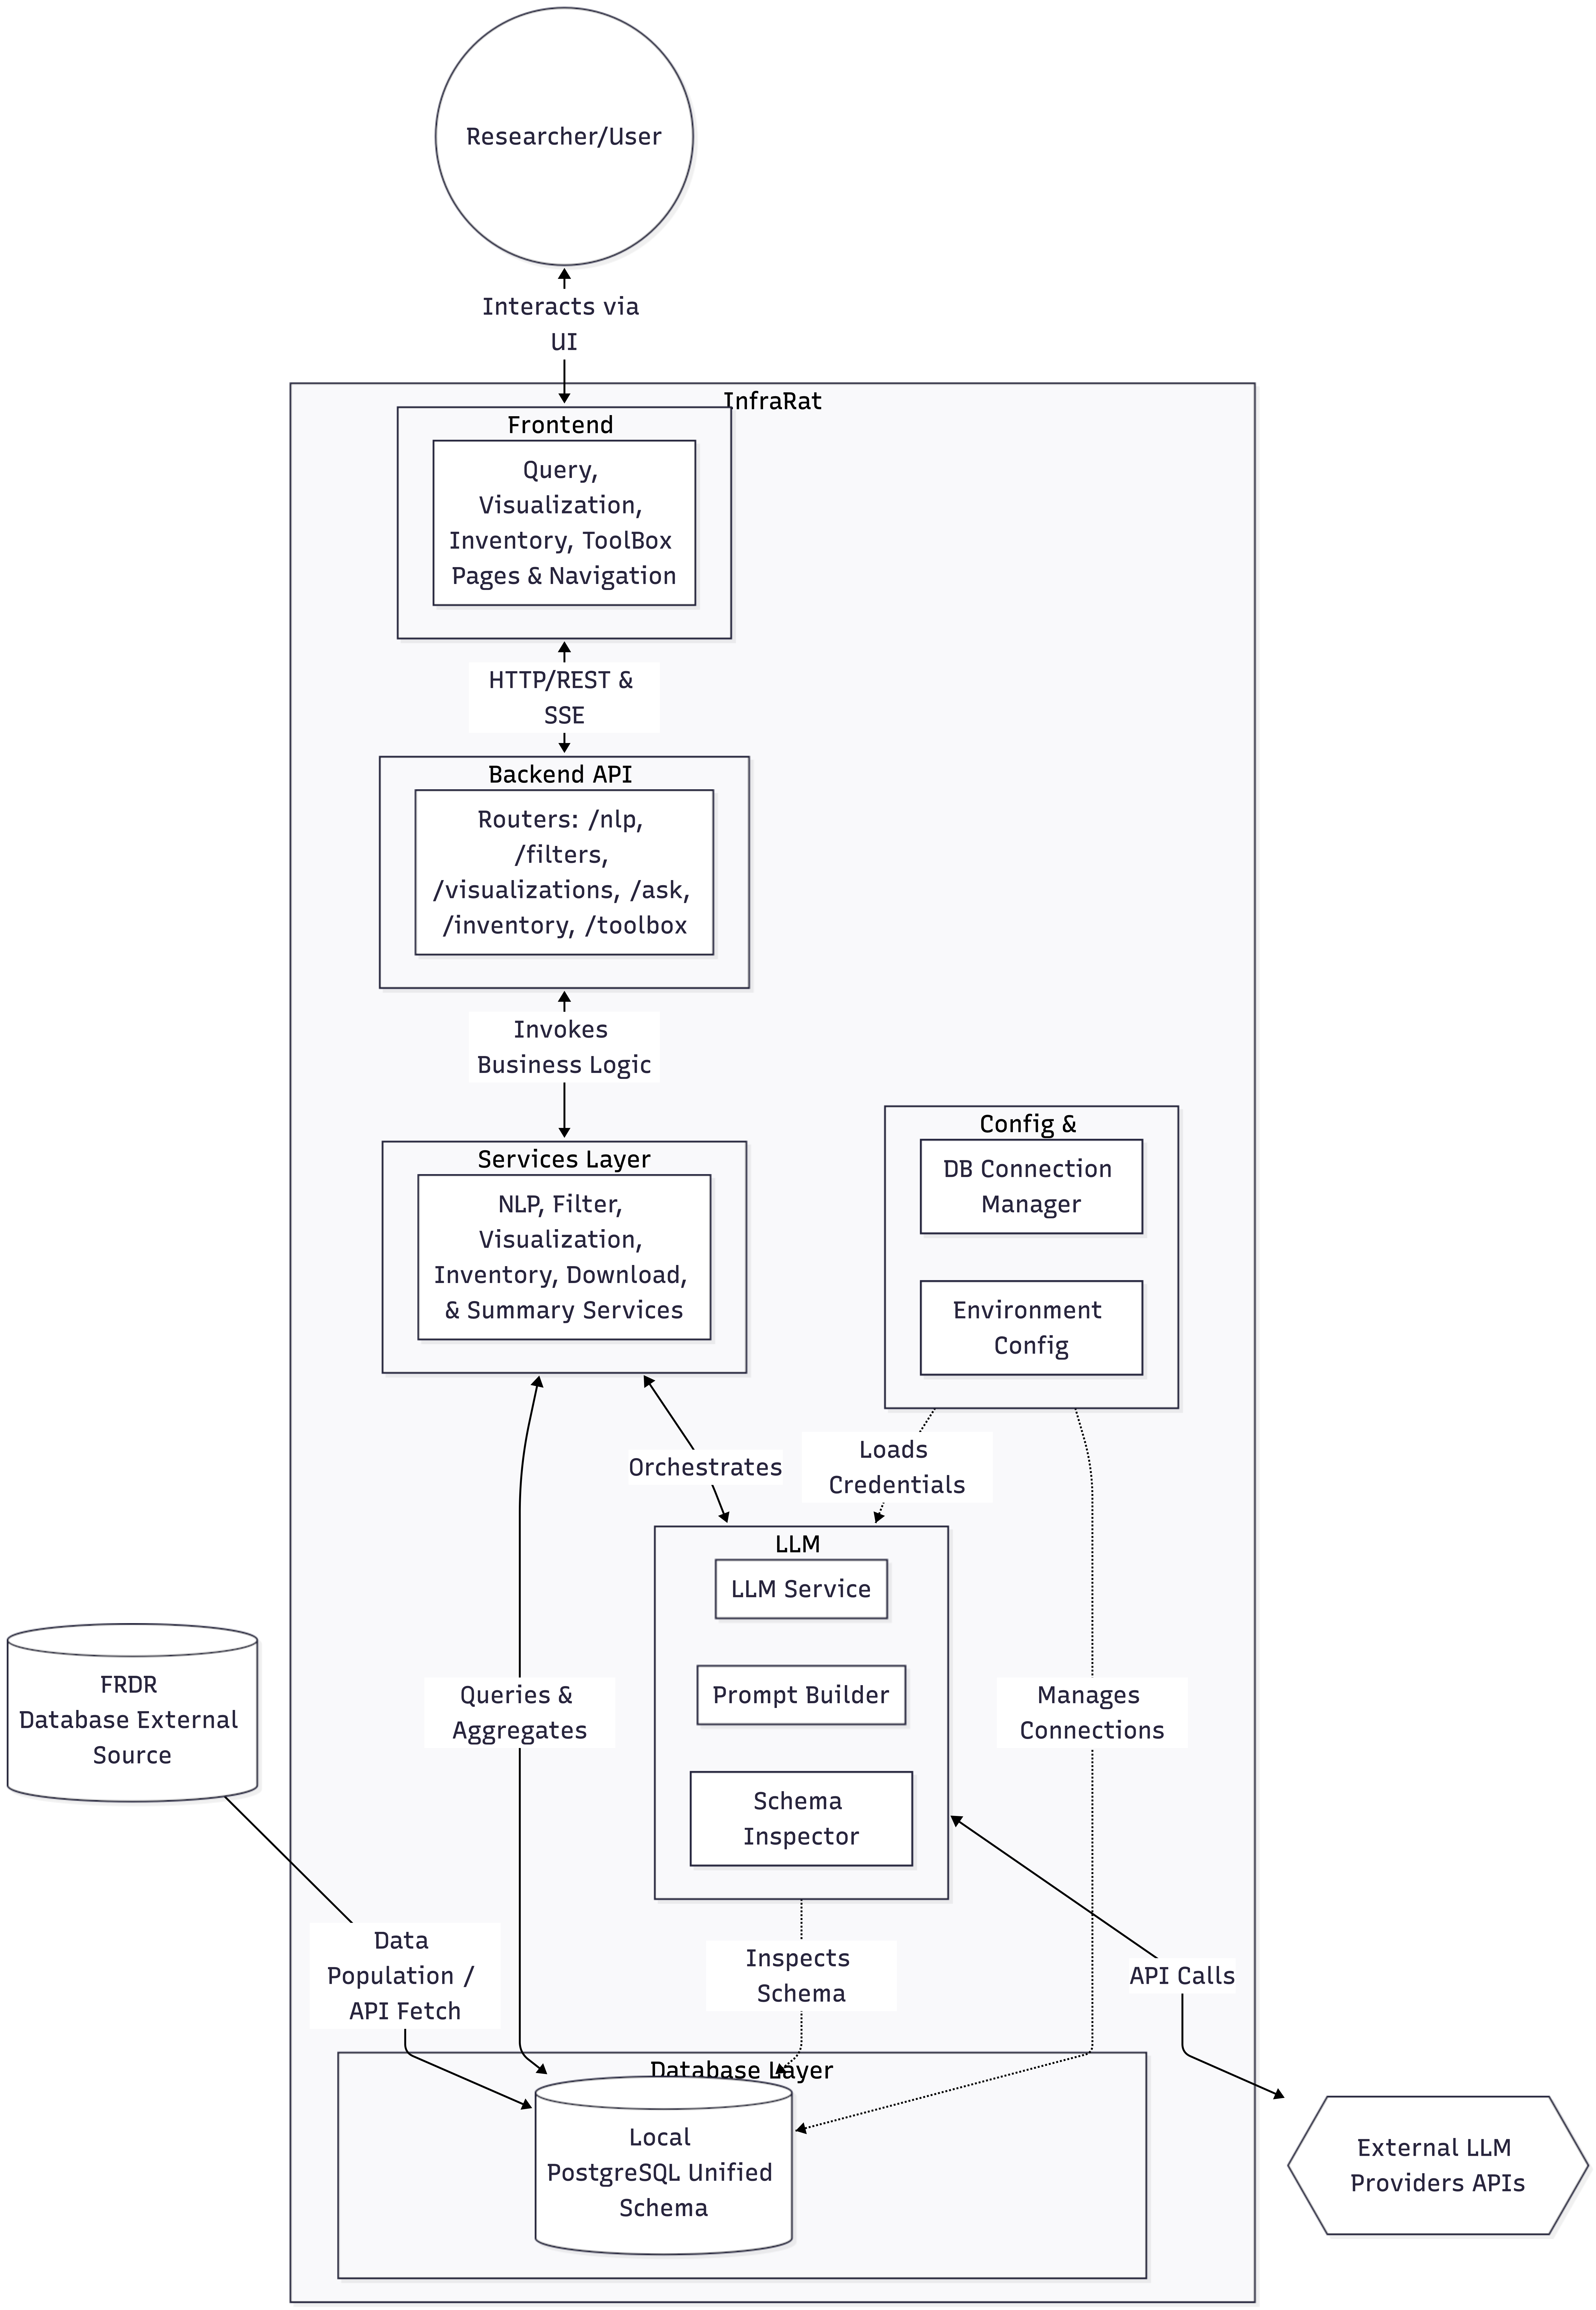
\includegraphics[width=1.1\textwidth]{SystemBoundariesDiagram.png}%
    }
    \caption{System Boundaries Diagram}
    \label{fig:SystemBoundaries}
\end{figure}

\section{Critical Assumptions}


\begin{enumerate}
    \item FRDR API Availability
    \item[] It is assumed that the FRDR repository and corresponding API will remain accessibile and availabile throughout the lifetime of the product. API outages and/or other lapses in availability of this resource will be considered outside of the team's control. To mitigate potential unavailability, the system will implement local data caching for frequently accessed metadata, periodic snapshots of key datasets, and support for hybrid storage models (e.g., mirroring critical data locally for offline access). If FRDR becomes permanently unavailable, the system can fall back to cached data with clear user notifications about data freshness. 
    \item Read-Only Data Access
    \item[] It is assumed that the system will access the FRDR dataset solely in a read-only manner. Therefore, the system will not add, modify, or delete data from the source repository. 
    \item Minimum System Access Standards
    \item[] It is assumed that a user will access the system from a modern browser with JavaScript enabled. 
    \item Source Data Integrity 
    \item [] The system assumes that the individual data objects are accurate and correctly-labeled, therefore the corerrectness of experiments drawn from the platform is independent of the FRDR. 
\end{enumerate}

\section{Failure Mode and Effect Analysis}

\subsection{Hazards Considered Out of Scope}

\begin{itemize}
    \item The FRDR domain goes down for reasons such as maintenance or an outage (justification: This is managed by an external provider, Digital Research Alliance of Canada, and is beyond the team's control; however, the system includes monitoring and user notifications for such events).
    \item The FRDR repository or a subset of it is lost or corrupted (justification: Data preservation is handled by FRDR's infrastructure with redundant storage and backups; the system assumes data integrity but cannot prevent or recover from FRDR-level failures).
    \item Addition, modification, or deletion of FRDR data by an authorized user (justification: The system operates in read-only mode and does not provide data modification capabilities; changes to FRDR are performed externally by data owners like Dr. Szechtman).
    \item Pre-existing errors in FRDR metadata and mislabeled entries (justification: The system assumes source data integrity as per ASSUMPTION.7 in the SRS; systematic errors would require FRDR-level corrections, not system-level fixes).
    \item The user misuses data by making an error in interpreting information through the system's data visualizer (justification: While system design can mitigate this through clear labeling and tooltips, ultimate data interpretation is a user responsibility; the system provides accurate data but cannot control how users analyze it).
    \item User experience affected by local system issues such as slow internet or failing hardware (justification: The system requires minimum standards (modern browser, JavaScript) but cannot control user-side infrastructure; users on legacy systems may experience reduced functionality as noted in ASSUMPTION.6).
\end{itemize}

\subsection{Failure Modes and Effect Analysis Table}

\begin{longtblr}[
  caption = {Severity Criteria Table},
  label = {TblSeverityCriteria},
]{
  colspec = {| Q[c,2cm] | Q[c,2cm] | Q[c,7cm]|}, 
  rowhead = 1,          
  hlines,               
}
    \textbf{Quantitative Score} & \textbf{Qualitative Score} & \textbf{Definition} \\
   
    1 & None & No impact on functionality, usability, or reliability \\
    
    2 & Minimal & Small cosmetic or display inconvenience, negligible effect on usability \\
  
    3 & Moderate & Noticeable regression in system usability, still functional but reduced performance  \\
  
    4 & High & Significant impact on functionality but there is a temporary workaround, harmful for productivity but not halting \\

    5 & Severe & Major impact on system fidelity with data/analysis errors causing users to lose confidence in results \\
 
    6 & Critical & Major functional malfunction for core tasks such as searching, filtering, or visualizing. Users cannot complete primary workflows  \\
  
    7 & Catastrophic & System is entirely inoperable or research integrity compromised by materially misleading researchers with invalid results \\

\end{longtblr}


\begin{longtblr}[
  caption = {Occurrence Criteria Table},
  label = {TblOccurrenceCriteria},
]{
  colspec = {|Q[c,2cm] | Q[c,2cm] | Q[c,7cm]|}, 
  rowhead = 1,          
  hlines,               
}
    \textbf{Quantitative Score} & \textbf{Qualitative Score} & \textbf{Probability} \\
   
    1 & Extremely Rare & $<0.1\%$ \\
    
    2 & Rare & $0.1-0.5\%$ \\
    
    3 & Very Low & $0.5-2\%$ \\
   
    4 & Low & $2-5\%$ \\
    
    5 & Somewhat Moderate & $5-10\%$ \\
    
    6 & Moderate & $10-30\%$ \\
   
    7 & Moderately High & $30-50\%$ \\
   
    8 & High & $50-75\%$ \\
   
    9 & Very Often & $75-90\%$ \\
  
    10 & Almost Expected & $>90\%$ \\

\end{longtblr}

 \begin{longtblr}[
  caption = {Detection Criteria Table},
  label = {TblDetectionCriteria},
]{
  colspec = {|Q[c,2cm] | Q[c,2cm] | Q[c,7cm]|}, 
  rowhead = 1,          
  hlines,               
}

    \textbf{Quantitative Score} & \textbf{Qualitative Score} & \textbf{Detectability} \\
    1 & Certain & $100\%$ Detection \\
    
    2 & Almost certain & $90\%$ Detection \\
   
    3 & High & $75\%$ Detection \\
   
    4 & Moderate & $50\%$ Detection \\
   
    5 & Low & $30\%$ Detection \\

    6 & Almost Impossible & $<10\%$ Detection \\

\end{longtblr}

\clearpage

\begin{figure}[h]
    \centering
    \includegraphics[width=1\textwidth]{FMEA Table 1.png}
    \caption{FMEA Table (Part 1)}
    \label{fig:TblFMEA1}
\end{figure}

\clearpage

\begin{figure}[h]
    \centering
    \includegraphics[width=1\textwidth]{FMEA Table 2.png}
    \caption{FMEA Table (Part 2)}
    \label{fig:TblFMEA2}
\end{figure}

\section{Safety and Security Requirements}

\subsection{Safety Requirements}
\par{The system does not directly involve physical safety or critical operations. However, to ensure data reliability and prevent unintended harm to research workflows, the following safety requirements have been identified:}
\begin{itemize}
    \item \textbf{SAF.R.1 -- Data Integrity Protection} \\
    \textbf{Description:} The system shall ensure that all query results are returned exactly as stored in the FRDR repository, without modification or corruption. \\
    \textbf{Rationale:} Prevents accidental misinterpretation of research data that could lead to invalid conclusions. \\
    \textbf{Fit Criterion:} Query results match the FRDR source files exactly, verified through checksum or metadata comparison.
    
    \item \textbf{SAF.R.2 -- Fault Isolation} \\
    \textbf{Description:} Failures in one component (e.g., NLP module) shall not compromise the operation of other system components. \\
    \textbf{Rationale:} Prevents cascading failures that could disrupt research sessions. \\
    \textbf{Fit Criterion:} The system remains operational when individual modules fail, with appropriate error messages.
    
    \item \textbf{SAF.R.3 -- Safe Handling of Large Data Sets} \\
    \textbf{Description:} The system shall prevent browsers from directly loading excessively large datasets, instead providing download or batch processing options. \\
    \textbf{Rationale:} Protects user devices from freezing or crashing during analysis. \\
    \textbf{Fit Criterion:} Queries exceeding size thresholds trigger warnings and offer alternative access methods.
\end{itemize}

\subsection{Security Requirements}
\begin{itemize}
    \item \textbf{SEC.R.1 -- Enhanced Input Validation} \\
    \textbf{Description:} All user inputs must go through validation to prevent inappropriate queries, code injection, or other malicious activity. \\
    \textbf{Rationale:} Prevents injection attacks and malformed queries from reaching backend services. \\
    \textbf{Fit Criterion:} All inputs are sanitized and penetration testing shows no injection vulnerabilities.
    
    \item \textbf{SEC.R.2 -- Access Logging} \\
    \textbf{Description:} All administrative actions, including deployment and maintenance, must be logged to provide traceability. \\
    \textbf{Rationale:} Ensures accountability and allows auditing of configuration changes. \\
    \textbf{Fit Criterion:} 100\% of administrative actions are logged with timestamps and stored securely.
    
    \item \textbf{SEC.R.3 -- Dependency Monitoring} \\
    \textbf{Description:} The system shall scan and monitor open-source frameworks, dependencies, and libraries for security vulnerabilities and update them regularly. \\
    \textbf{Rationale:} Protects against exploitation through known vulnerabilities in third-party components. \\
    \textbf{Fit Criterion:} Automated scans show no unresolved high-severity vulnerabilities older than 14 days.
    
    \item \textbf{SEC.R.4 -- Incident Documentation} \\
    \textbf{Description:} The team shall maintain documentation outlining procedures for responding to security incidents, including roles, notifications, and mitigation timelines. \\
    \textbf{Rationale:} Ensures coordinated and timely responses to potential security incidents. \\
    \textbf{Fit Criterion:} Incident response documentation exists, is reviewed regularly, and defines clear escalation steps.
    
    \item \textbf{SEC.R.5 -- Safe File Downloads} \\
    \textbf{Description:} All downloadable files shall be scanned for malware and saved with appropriate protection to safeguard user environments. \\
    \textbf{Rationale:} Prevents the distribution of malicious or corrupted files to researchers. \\
    \textbf{Fit Criterion:} All files pass malware scanning before being made available for download.
\end{itemize}


\pagebreak

\section{Roadmap}


\textbf{Scheduled for Implementation}
\par{The following safety and security requirements have been prioritized by safety and security impact and relevance to project stakeholders. }

\begin{table*}[h!]
\begin{tabularx}{\textwidth}{ X X X } 
    \textbf{ID} & \textbf{Description} & \textbf{Timing} \\
    \hline
    SAF.R.1 & Data Integrity Protection &  During Backend API integration phase   \\
    \hline 
    SAF.R.2 & Fault Isolation & During Integration Testing phase \\ 
    \hline 
    SAF.R.3 & Safe Handling  of Large Data Sets &  During backend query module implementation \\
    \hline
    SEC.R.1 & Input Validation & During frontend and API design phase \\ 
    \hline 
    SEC.R.3 & Dependency Monitoring & Immediately during development phase. \\
    \hline 
\end{tabularx}
\end{table*}



\vspace{\baselineskip}

\textbf{Deferred and Future Requirements}

\par{
The following Safety and Security requirements will not be implemented as part of the capstone due to time constraints and prioritization, however they are noted for future relevance.  
}

\begin{table*}[h!]
\begin{tabularx}{\textwidth}{ l X X } 
    \textbf{ID} & \textbf{Description} & \textbf{Justification} \\
    \hline
    SEC.R.2  & Access Logging & Low business value to client  \\
    \hline
    SEC.R.4 & Incident Documentation and response procedures & To be implemented by future maintainers of system.  \\
    \hline
        SEC.R.5 & Safe File Downloads & Out of scope for current implementation. Not a priority due to the fixed nature of FRDR data.   \\
    \hline
\end{tabularx}
\end{table*}


\newpage{}

\section*{Appendix --- Reflection}

\input{../Reflection.tex}

\begin{enumerate}
    \item What went well while writing this deliverable? 
    \item What pain points did you experience during this deliverable, and how
    did you resolve them?
    \item Which of your listed risks had your team thought of before this
    deliverable, and which did you think of while doing this deliverable? For
    the latter ones (ones you thought of while doing the Hazard Analysis), how
    did they come about?
    \item Other than the risk of physical harm (some projects may not have any
    appreciable risks of this form), list at least 2 other types of risk in
    software products. Why are they important to consider?
\end{enumerate}

\section{Team Reflection}
\begin{enumerate}
    \item \textbf{What went well while writing this deliverable?} \\
    One aspect that went well was our ability to clearly define and structure the requirements. We had already spoken to the client beforehand, so most of the functional requirements were straightforward to articulate. Additionally, the team collaborated efficiently, dividing the work logically at the start of the Hazard Analysis and reviewing each other's sections to maintain consistency.

    \item \textbf{What pain points did you experience during this deliverable, and how did you resolve them?} \\
    One challenge was distinguishing between functional and non-functional requirements. The client's input primarily focused on functionality and interface expectations, so we had to determine additional non-functional software-related requirements ourselves. We resolved this by holding a short internal meeting to clarify definitions and cross-check each requirement category for accuracy.

    \item \textbf{Which of your listed risks had your team thought of before this deliverable, and which did you think of while doing this deliverable? For the latter ones, how did they come about?} \\
    Before starting, we had already identified risks related to physical harm and basic security concerns. However, while completing the hazard analysis, we recognized additional risks such as data integrity issues and usability-related failures. These arose as we analyzed system interactions in more depth and considered edge cases that were not initially obvious.

    \item \textbf{Other than the risk of physical harm, list at least 2 other types of risk in software products. Why are they important to consider?} 
    \begin{itemize}
        \item \textbf{Security Risks:} These include unauthorized access, data breaches, or injection attacks. They are critical because they can compromise sensitive user information and damage system integrity.
        \item \textbf{Reliability Risks:} These involve the system failing to perform as expected under normal or stress conditions. Considering these is essential to ensure system stability and maintain user trust.
    \end{itemize}
\end{enumerate}

\end{document}
